% Options for packages loaded elsewhere
\PassOptionsToPackage{unicode}{hyperref}
\PassOptionsToPackage{hyphens}{url}
\PassOptionsToPackage{dvipsnames,svgnames,x11names}{xcolor}
%
\documentclass[
  letterpaper,
  DIV=11,
  numbers=noendperiod]{scrartcl}

\usepackage{amsmath,amssymb}
\usepackage{iftex}
\ifPDFTeX
  \usepackage[T1]{fontenc}
  \usepackage[utf8]{inputenc}
  \usepackage{textcomp} % provide euro and other symbols
\else % if luatex or xetex
  \usepackage{unicode-math}
  \defaultfontfeatures{Scale=MatchLowercase}
  \defaultfontfeatures[\rmfamily]{Ligatures=TeX,Scale=1}
\fi
\usepackage{lmodern}
\ifPDFTeX\else  
    % xetex/luatex font selection
\fi
% Use upquote if available, for straight quotes in verbatim environments
\IfFileExists{upquote.sty}{\usepackage{upquote}}{}
\IfFileExists{microtype.sty}{% use microtype if available
  \usepackage[]{microtype}
  \UseMicrotypeSet[protrusion]{basicmath} % disable protrusion for tt fonts
}{}
\makeatletter
\@ifundefined{KOMAClassName}{% if non-KOMA class
  \IfFileExists{parskip.sty}{%
    \usepackage{parskip}
  }{% else
    \setlength{\parindent}{0pt}
    \setlength{\parskip}{6pt plus 2pt minus 1pt}}
}{% if KOMA class
  \KOMAoptions{parskip=half}}
\makeatother
\usepackage{xcolor}
\setlength{\emergencystretch}{3em} % prevent overfull lines
\setcounter{secnumdepth}{5}
% Make \paragraph and \subparagraph free-standing
\makeatletter
\ifx\paragraph\undefined\else
  \let\oldparagraph\paragraph
  \renewcommand{\paragraph}{
    \@ifstar
      \xxxParagraphStar
      \xxxParagraphNoStar
  }
  \newcommand{\xxxParagraphStar}[1]{\oldparagraph*{#1}\mbox{}}
  \newcommand{\xxxParagraphNoStar}[1]{\oldparagraph{#1}\mbox{}}
\fi
\ifx\subparagraph\undefined\else
  \let\oldsubparagraph\subparagraph
  \renewcommand{\subparagraph}{
    \@ifstar
      \xxxSubParagraphStar
      \xxxSubParagraphNoStar
  }
  \newcommand{\xxxSubParagraphStar}[1]{\oldsubparagraph*{#1}\mbox{}}
  \newcommand{\xxxSubParagraphNoStar}[1]{\oldsubparagraph{#1}\mbox{}}
\fi
\makeatother


\providecommand{\tightlist}{%
  \setlength{\itemsep}{0pt}\setlength{\parskip}{0pt}}\usepackage{longtable,booktabs,array}
\usepackage{calc} % for calculating minipage widths
% Correct order of tables after \paragraph or \subparagraph
\usepackage{etoolbox}
\makeatletter
\patchcmd\longtable{\par}{\if@noskipsec\mbox{}\fi\par}{}{}
\makeatother
% Allow footnotes in longtable head/foot
\IfFileExists{footnotehyper.sty}{\usepackage{footnotehyper}}{\usepackage{footnote}}
\makesavenoteenv{longtable}
\usepackage{graphicx}
\makeatletter
\def\maxwidth{\ifdim\Gin@nat@width>\linewidth\linewidth\else\Gin@nat@width\fi}
\def\maxheight{\ifdim\Gin@nat@height>\textheight\textheight\else\Gin@nat@height\fi}
\makeatother
% Scale images if necessary, so that they will not overflow the page
% margins by default, and it is still possible to overwrite the defaults
% using explicit options in \includegraphics[width, height, ...]{}
\setkeys{Gin}{width=\maxwidth,height=\maxheight,keepaspectratio}
% Set default figure placement to htbp
\makeatletter
\def\fps@figure{htbp}
\makeatother

\KOMAoption{captions}{tableheading}
\makeatletter
\@ifpackageloaded{caption}{}{\usepackage{caption}}
\AtBeginDocument{%
\ifdefined\contentsname
  \renewcommand*\contentsname{Table of contents}
\else
  \newcommand\contentsname{Table of contents}
\fi
\ifdefined\listfigurename
  \renewcommand*\listfigurename{List of Figures}
\else
  \newcommand\listfigurename{List of Figures}
\fi
\ifdefined\listtablename
  \renewcommand*\listtablename{List of Tables}
\else
  \newcommand\listtablename{List of Tables}
\fi
\ifdefined\figurename
  \renewcommand*\figurename{Figure}
\else
  \newcommand\figurename{Figure}
\fi
\ifdefined\tablename
  \renewcommand*\tablename{Table}
\else
  \newcommand\tablename{Table}
\fi
}
\@ifpackageloaded{float}{}{\usepackage{float}}
\floatstyle{ruled}
\@ifundefined{c@chapter}{\newfloat{codelisting}{h}{lop}}{\newfloat{codelisting}{h}{lop}[chapter]}
\floatname{codelisting}{Listing}
\newcommand*\listoflistings{\listof{codelisting}{List of Listings}}
\makeatother
\makeatletter
\makeatother
\makeatletter
\@ifpackageloaded{caption}{}{\usepackage{caption}}
\@ifpackageloaded{subcaption}{}{\usepackage{subcaption}}
\makeatother

\ifLuaTeX
  \usepackage{selnolig}  % disable illegal ligatures
\fi
\usepackage{bookmark}

\IfFileExists{xurl.sty}{\usepackage{xurl}}{} % add URL line breaks if available
\urlstyle{same} % disable monospaced font for URLs
\hypersetup{
  pdftitle={Summer School I},
  colorlinks=true,
  linkcolor={blue},
  filecolor={Maroon},
  citecolor={Blue},
  urlcolor={Blue},
  pdfcreator={LaTeX via pandoc}}


\title{Summer School I}
\author{}
\date{}

\begin{document}
\maketitle

\renewcommand*\contentsname{Table of contents}
{
\hypersetup{linkcolor=}
\setcounter{tocdepth}{3}
\tableofcontents
}

\begin{center}

\includegraphics[width=3.39583in,height=\textheight]{images/ss logo.jpg}
\end{center}

\textbf{Location:} Benicàssim, Spain

\textbf{Host:} University of Jaume I

\textbf{Project :}
\href{https://experience.arcgis.com/experience/2dbbd653dec545038635c3ebe36d8432/page/About-Nextcity}{NextCity}

\textbf{Date :} June 3--6, 2025

In June 2025, I participated in the \textbf{NextCity Summer School and
Thematic Workshop}, a program combining theory and hands-on experience
in \textbf{digital twins}, \textbf{GeoAI} and \textbf{3D GIS}. Hosted in
the beautiful town of Benicàssim, Spain, and organized under the
NextCity project, the event brought together students, researchers, and
professionals to explore the future of urban innovation.

\subsection{\texorpdfstring{\textbf{Jun 3-4 : Summer school : Concepts
\&
Theory}}{Jun 3-4 : Summer school : Concepts \& Theory}}\label{jun-3-4-summer-school-concepts-theory}

The first two days of the summer school were on the theoretical aspect
of Digital Twins and smart city technologies.

\textbf{Day 1 -- Technologies and tools for developing digital twins}

The first day of the summer school, led by \textbf{Florian Fischer}
\textbf{(Esri Germany)}, was on understanding the technologies that
develop digital twin systems, with a focus on reality mapping, real-time
data integration, and 3D model generation using ESRI tools \emph{ArcGIS
Reality for ArcGIS Pro and ArcGIS Reality Studio.}

We began by exploring \emph{aerial triangulation and dense image
matching techniques}, which form the basis of accurate 3D
reconstruction. These methods enable the generation of high-resolution
spatial models from overlapping images, ensuring both precision and
realism. A particularly fascinating component was the process of 3D-mesh
generation, where algorithms automatically filter out moving objects,
resulting in clean urban representations, essential for maintaining
consistency in urban simulations.

Another advanced rendering technique presented was the use of
\emph{Gaussian splats}, an innovative approach for visualizing complex
3D environments with photorealistic quality, particularly effective when
modeling natural textures or urban facades. In parallel, we also
examined the availability and value of open lidar datasets, such as
those made publicly accessible in the Netherlands, which highlight how
national-level open data policies can support digital twin innovation.

Collectively, these technologies demonstrated how spatial data, when
combined with the right analytical tools, can be transformed into
dynamic, high-resolution urban models. These models serve not only as
visual representations but also as data-rich platforms for analysis,
simulation, and real-time decision-making.

\textbf{Day 2 -- AI and prediction in Digital Twins}

The second day of the summer school was on the integration of AI in the
digital twin ecosystem. Led by \textbf{Minerva Centeno from Esri Spain},
the morning session introduced GeoAI, highlighting how machine learning
and spatial analysis are converging to enhance decision-making and
automate workflows in geospatial applications.

A central focus was the use of deep learning within ArcGIS, particularly
in generating unbiased \emph{True Ortho imagery}. Instead of relying
solely on traditional datasets like OpenStreetMap (OSM), models were
trained using Digital Surface Models (DSM) and slope data, reducing
potential bias and improving accuracy in height-sensitive environments.
Several key geoprocessing tools were explored, including \emph{Slope},
\emph{Extract by Attribute}, and \emph{Raster Solar Radiation},
demonstrating their utility in preparing data for AI pipelines.

We also looked into \emph{multi-resolution Level of Detail (LOD)
modeling}, covering a range from \emph{LOD 0 to 3.5}. This was
contextualized with real-world case studies, such as Hungary's LOD2
initiative which showcased national-scale 3D data production for
planning and governance.

A portion of the session was dedicated to the integration of open-source
AI libraries into ArcGIS, GEOAI, a framework that blends spatial
thinking with cutting-edge machine learning tools. We examined the use
of pre-trained models, including practical considerations like batch
size, cell resolution, and change detection. Among the tools discussed
were \emph{Text SAM (Segment Anything Model)}, \emph{Grounding DINO +
SAM} for text-guided segmentation, and techniques for crop
classification from time series data, all pointing toward more
intelligent and adaptable geospatial systems.

In the afternoon, \textbf{Joep Crompvoets from KU Leuven} led an
intriguing session on the impacts of 3D and AI-driven systems. His
discussion went beyond the technical to address digital governance in
geospatial systems, emphasizing the need for frameworks that evolve with
intelligent technologies. A compelling debate emerged around the
question: \textbf{\emph{``AI --- hype or hit?''}} This led to an
exploration of the philosophical divide between Symbolic AI and
Connectionist (Machine Learning) AI, and the growing efforts to
integrate both schools for more powerful systems. Key governance
takeaways included the importance of interdisciplinary collaboration and
balancing innovation with responsibility in designing future-ready
digital infrastructures.

\subsection{\texorpdfstring{\textbf{Jun 5-6: Thematic Workshop: From
Theory to
Practice}}{Jun 5-6: Thematic Workshop: From Theory to Practice}}\label{jun-5-6-thematic-workshop-from-theory-to-practice}

The second half of the program was dedicated to applying what we had
learned in a hands-on environment.

\textbf{Day 3 -- Fundamentals in 3D modelling}

Led by \textbf{Adrián Bautista (University of Jaume I)}, we focused on
the process of \emph{Blenderization}, the preparation and simplification
of 3D models for use in GIS environments. We began by working with CAD
models, which we imported into Blender to clean and optimize for GIS
workflows. These models were then georeferenced and visualized in ArcGIS
Pro, transforming raw architectural data into functional, spatially
aware 3D objects. This workflow showcased how design and geospatial
technologies converge in the digital twin pipeline.

We also explored \emph{ArcGIS Indoors}, introduced by \textbf{Nicolás
Luna (Univ. Jaume I),} to understand how interior spatial planning plays
a role in smart environments. This tool enables the visualization and
management of indoor spaces, setting the foundation for digital twin
solutions.

\textbf{Day 4 -- Indoor Mapping \& Smart Apps Development}

A continuation of the previous day session led by \textbf{Nicolás Luna
(Univ. Jaume I),} we extended our skills into \emph{indoor network
analysis}. We built indoor networks within a 3D building model using
\emph{ArcGIS Network Analyst}, simulating realistic routing scenarios ,
particularly relevant for large-scale indoor environments like airports,
hospitals, or shopping malls. We then published our results to ArcGIS
Online and developed an interactive web application combining 2D and 3D
maps, effectively communicating complex spatial relationships within
buildings.

\begin{quote}
\begin{quote}
\emph{Our Hands-On Output:}

\hfill\break
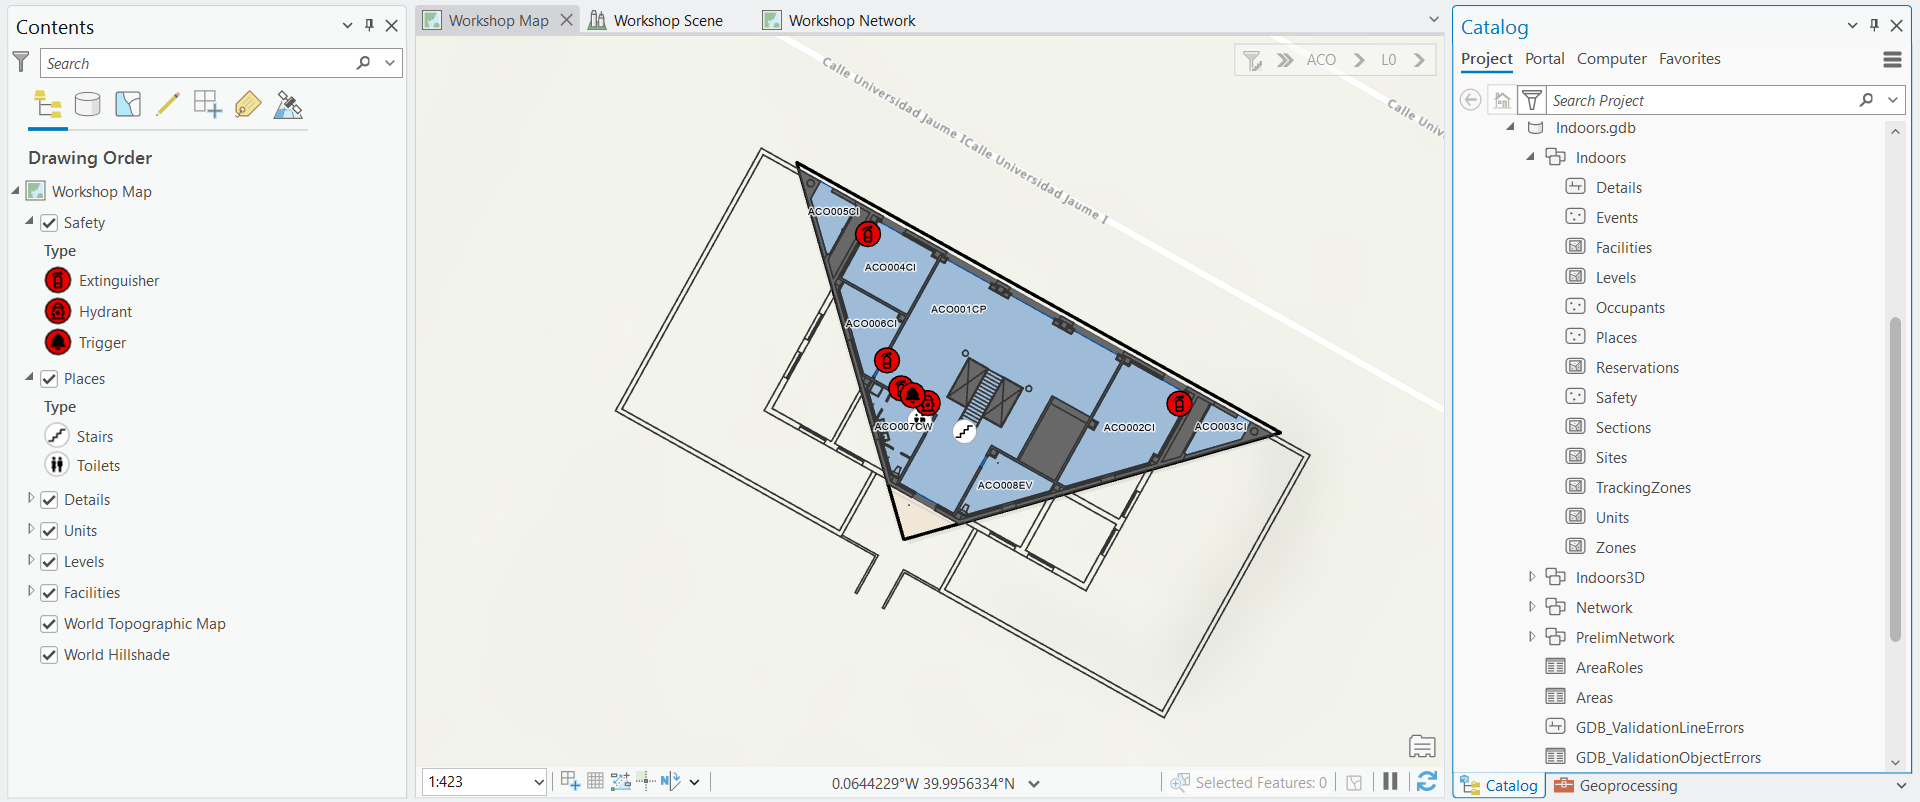
\includegraphics[width=7.95833in,height=\textheight]{images/indoor mapping.png}

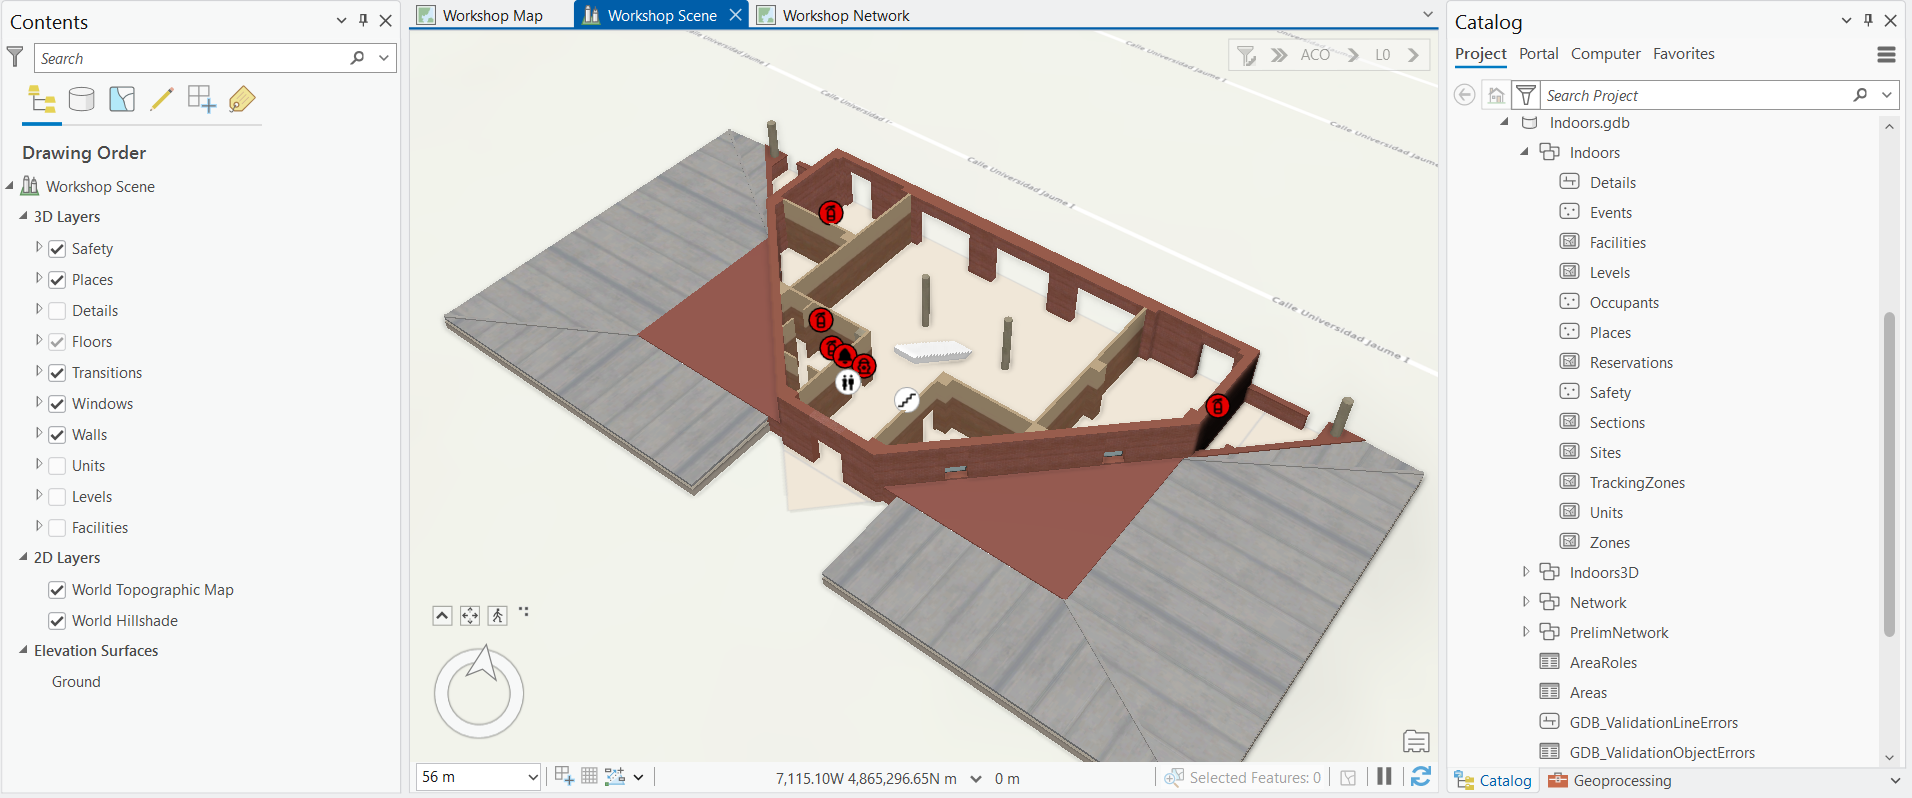
\includegraphics[width=7.97917in,height=\textheight]{images/3D result.png}

\emph{A detailed 3D model of a building we developed during the workshop
-- showcasing the full workflow from data to 3D visualization in ArcGIS
Pro.}
\end{quote}
\end{quote}

\subsection{\texorpdfstring{\textbf{Reflection}}{Reflection}}\label{reflection}

Participating in the summer school was a very enriching experience that
offered both technical depth and real-world perspective. We explored the
latest advancements in GIS, AI, and digital twin technologies, gaining
hands-on experience with tools like ArcGIS Reality, Blender, and ArcGIS
Indoors.

These exercises were not only technically rich, but also provided a
glimpse into real-world implementations. A good example was the digital
twin of the
\href{https://experience.arcgis.com/experience/6f6ff716866944ecaa2688888792864f/page/EN}{University
of Jaume I campus} , currently under development as part of their smart
campus initiative. This living model illustrates how digital twins can
support campus management, operations, and strategic planning.
Additionally, we learned about the NextCity project's vision to develop
a regional-scale digital twin for Lisbon's ZER region, underscoring the
increasing scale and importance of these technologies in urban and
regional planning.

For me, this was a foundational introduction to 3D mapping and digital
twin workflows. The combination of expert-led lectures and immersive
practical sessions helped bridge the gap between theory and application.
Most importantly, it initiated new ideas for applying digital twin
concepts to simulate Earth Observation scenarios such as flooding,
wildfire and landcover for monitoring.

Many thanks to the NextCity project and all its partners for organizing
this summer school. I would highly recommend this program to anyone
interested in geospatial technology, AI, or smart city development as
another edition is planned for next year, potentially in Belgium or
Portugal where the partner universities are located (\emph{look out for
their announcement for the location}).

\begin{quote}
\begin{quote}
\emph{The University of Jaume I digital twin}

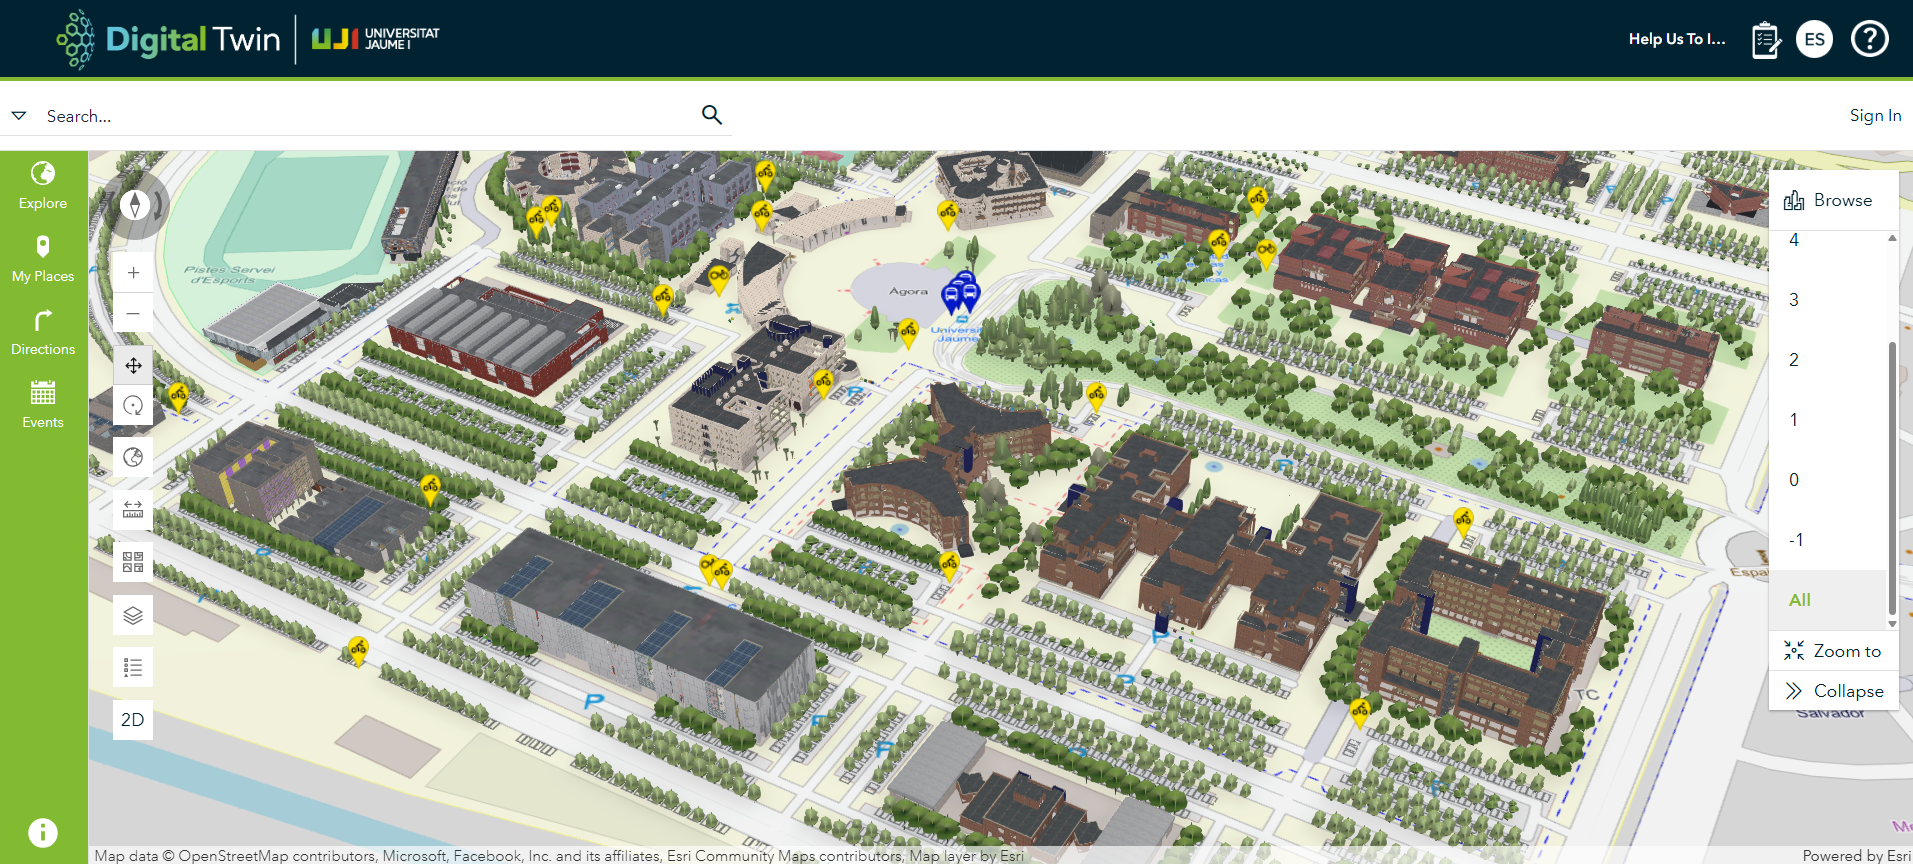
\includegraphics{images/clipboard-2844895517.png}

\emph{Memorable moments captured throughout the enriching ``Next City''
summer school.}

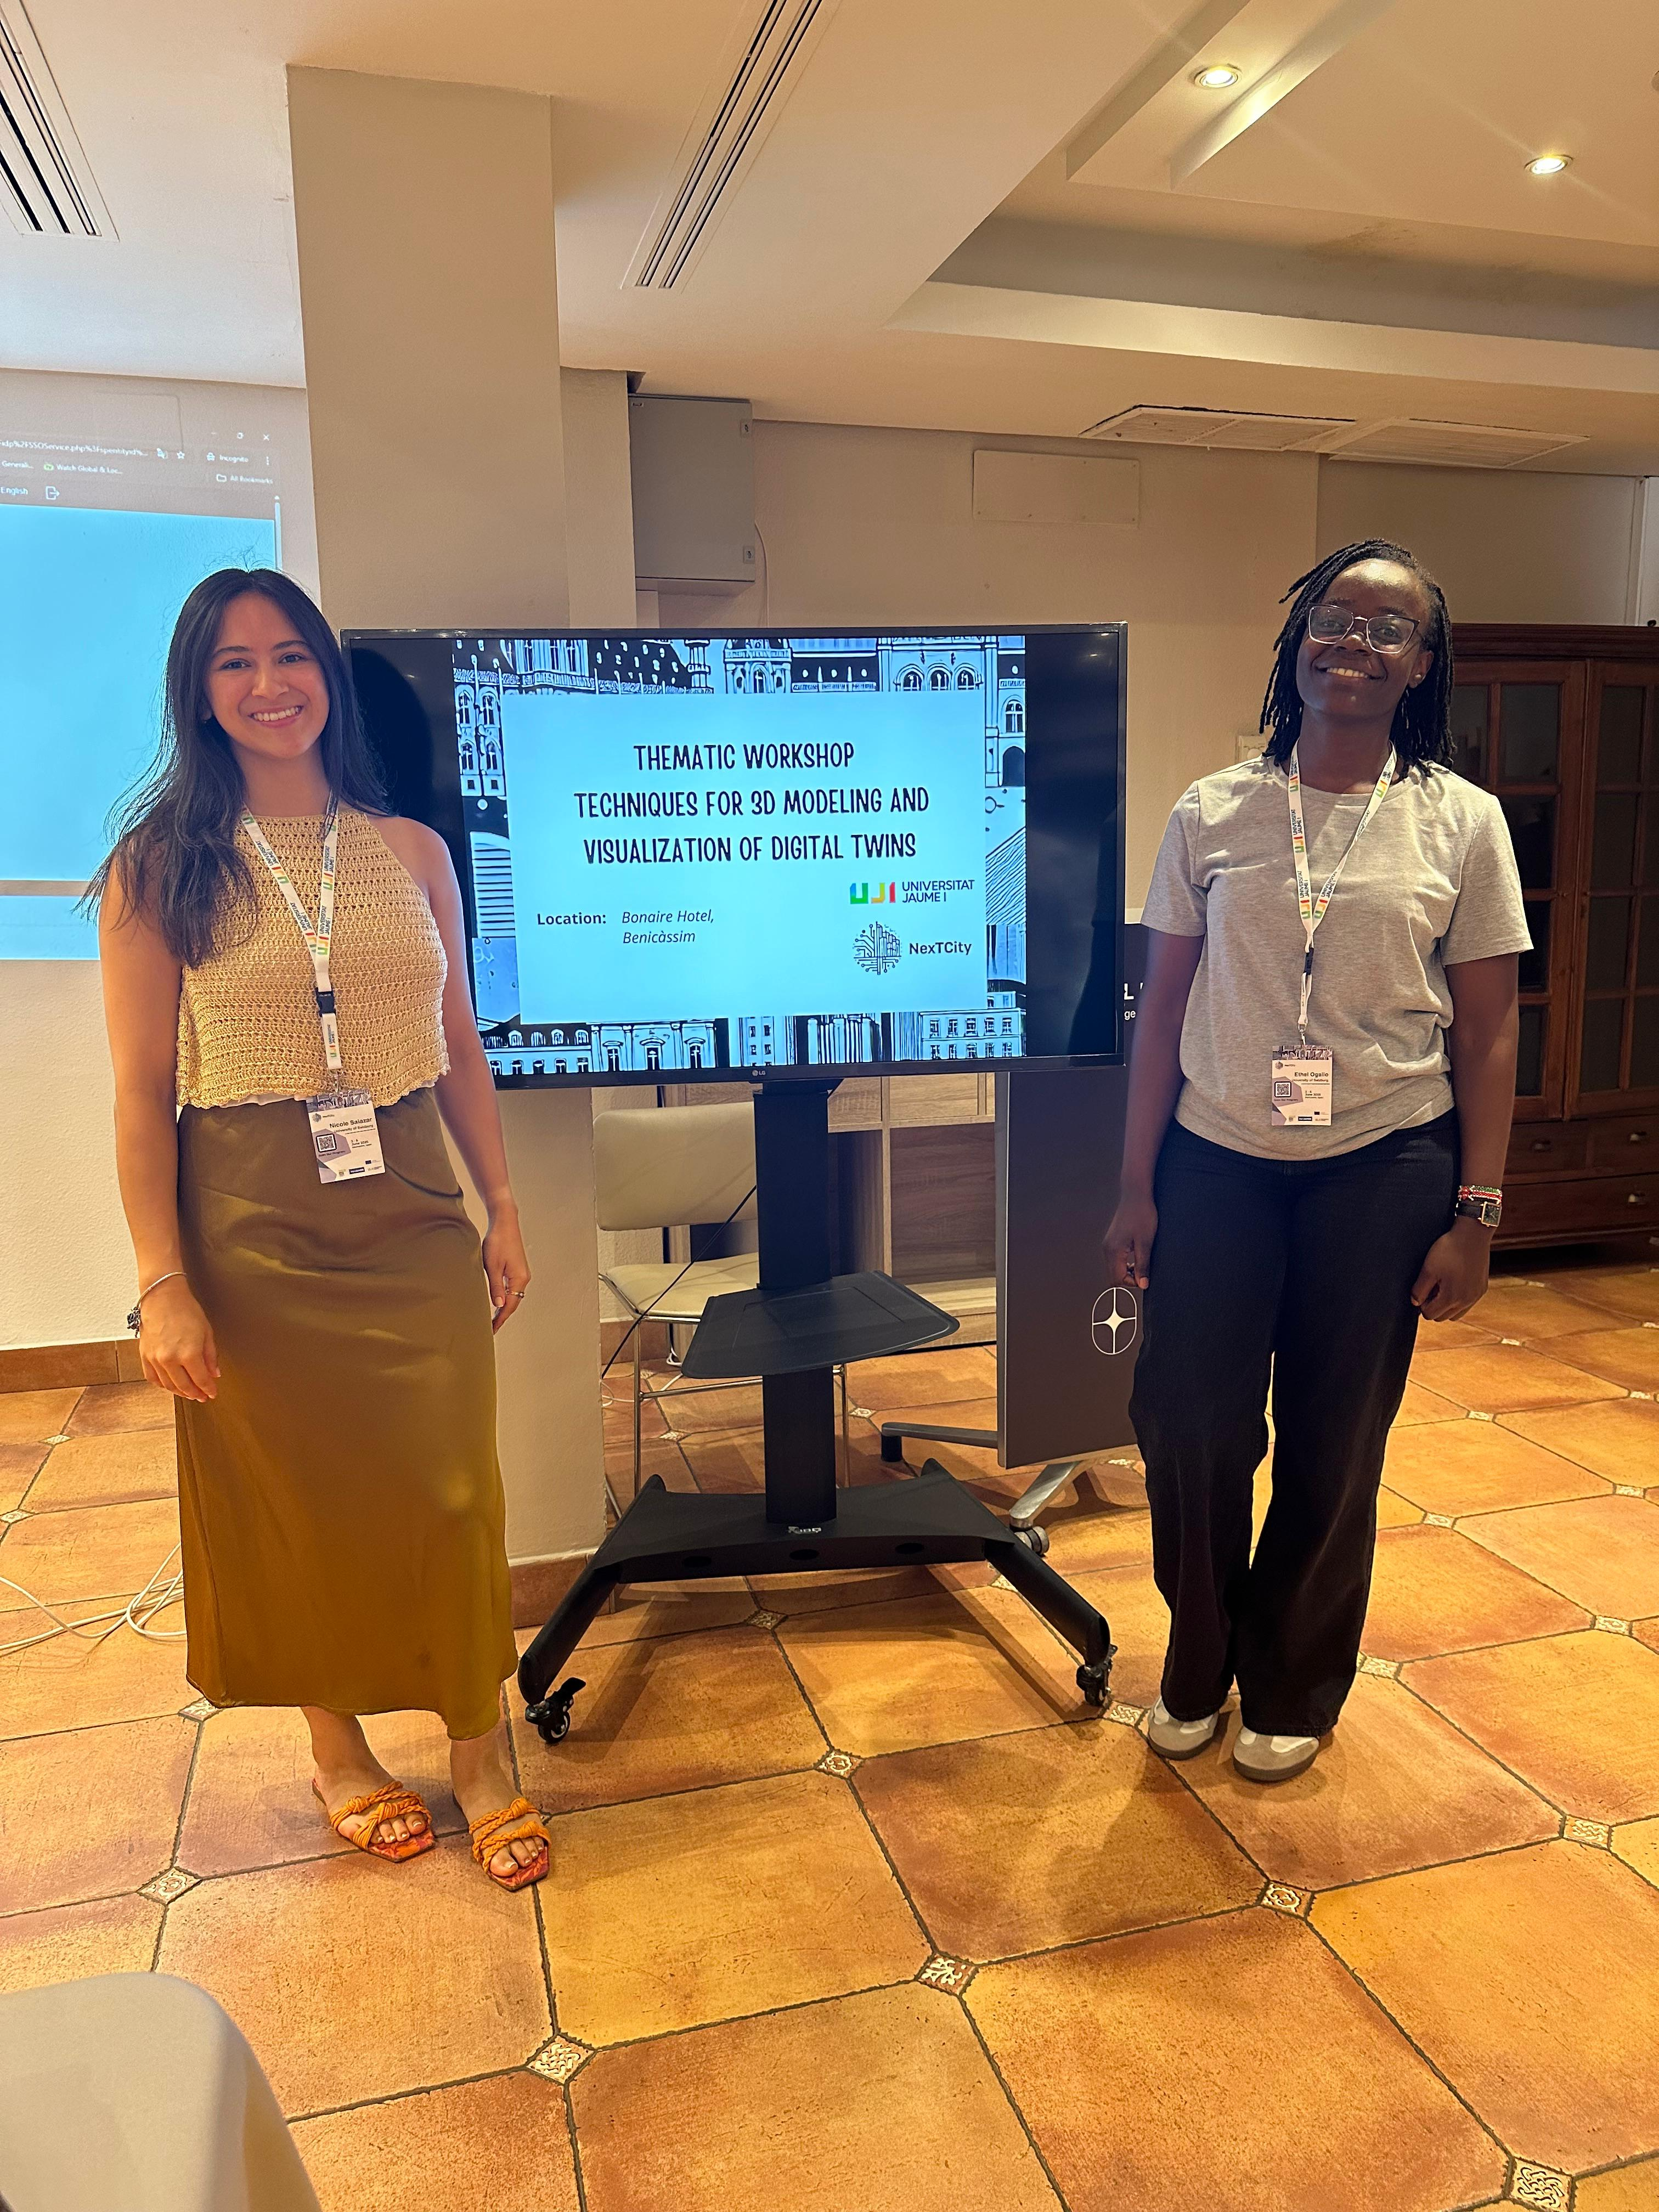
\includegraphics[width=3.30208in,height=\textheight]{images/cde rep.jpg}
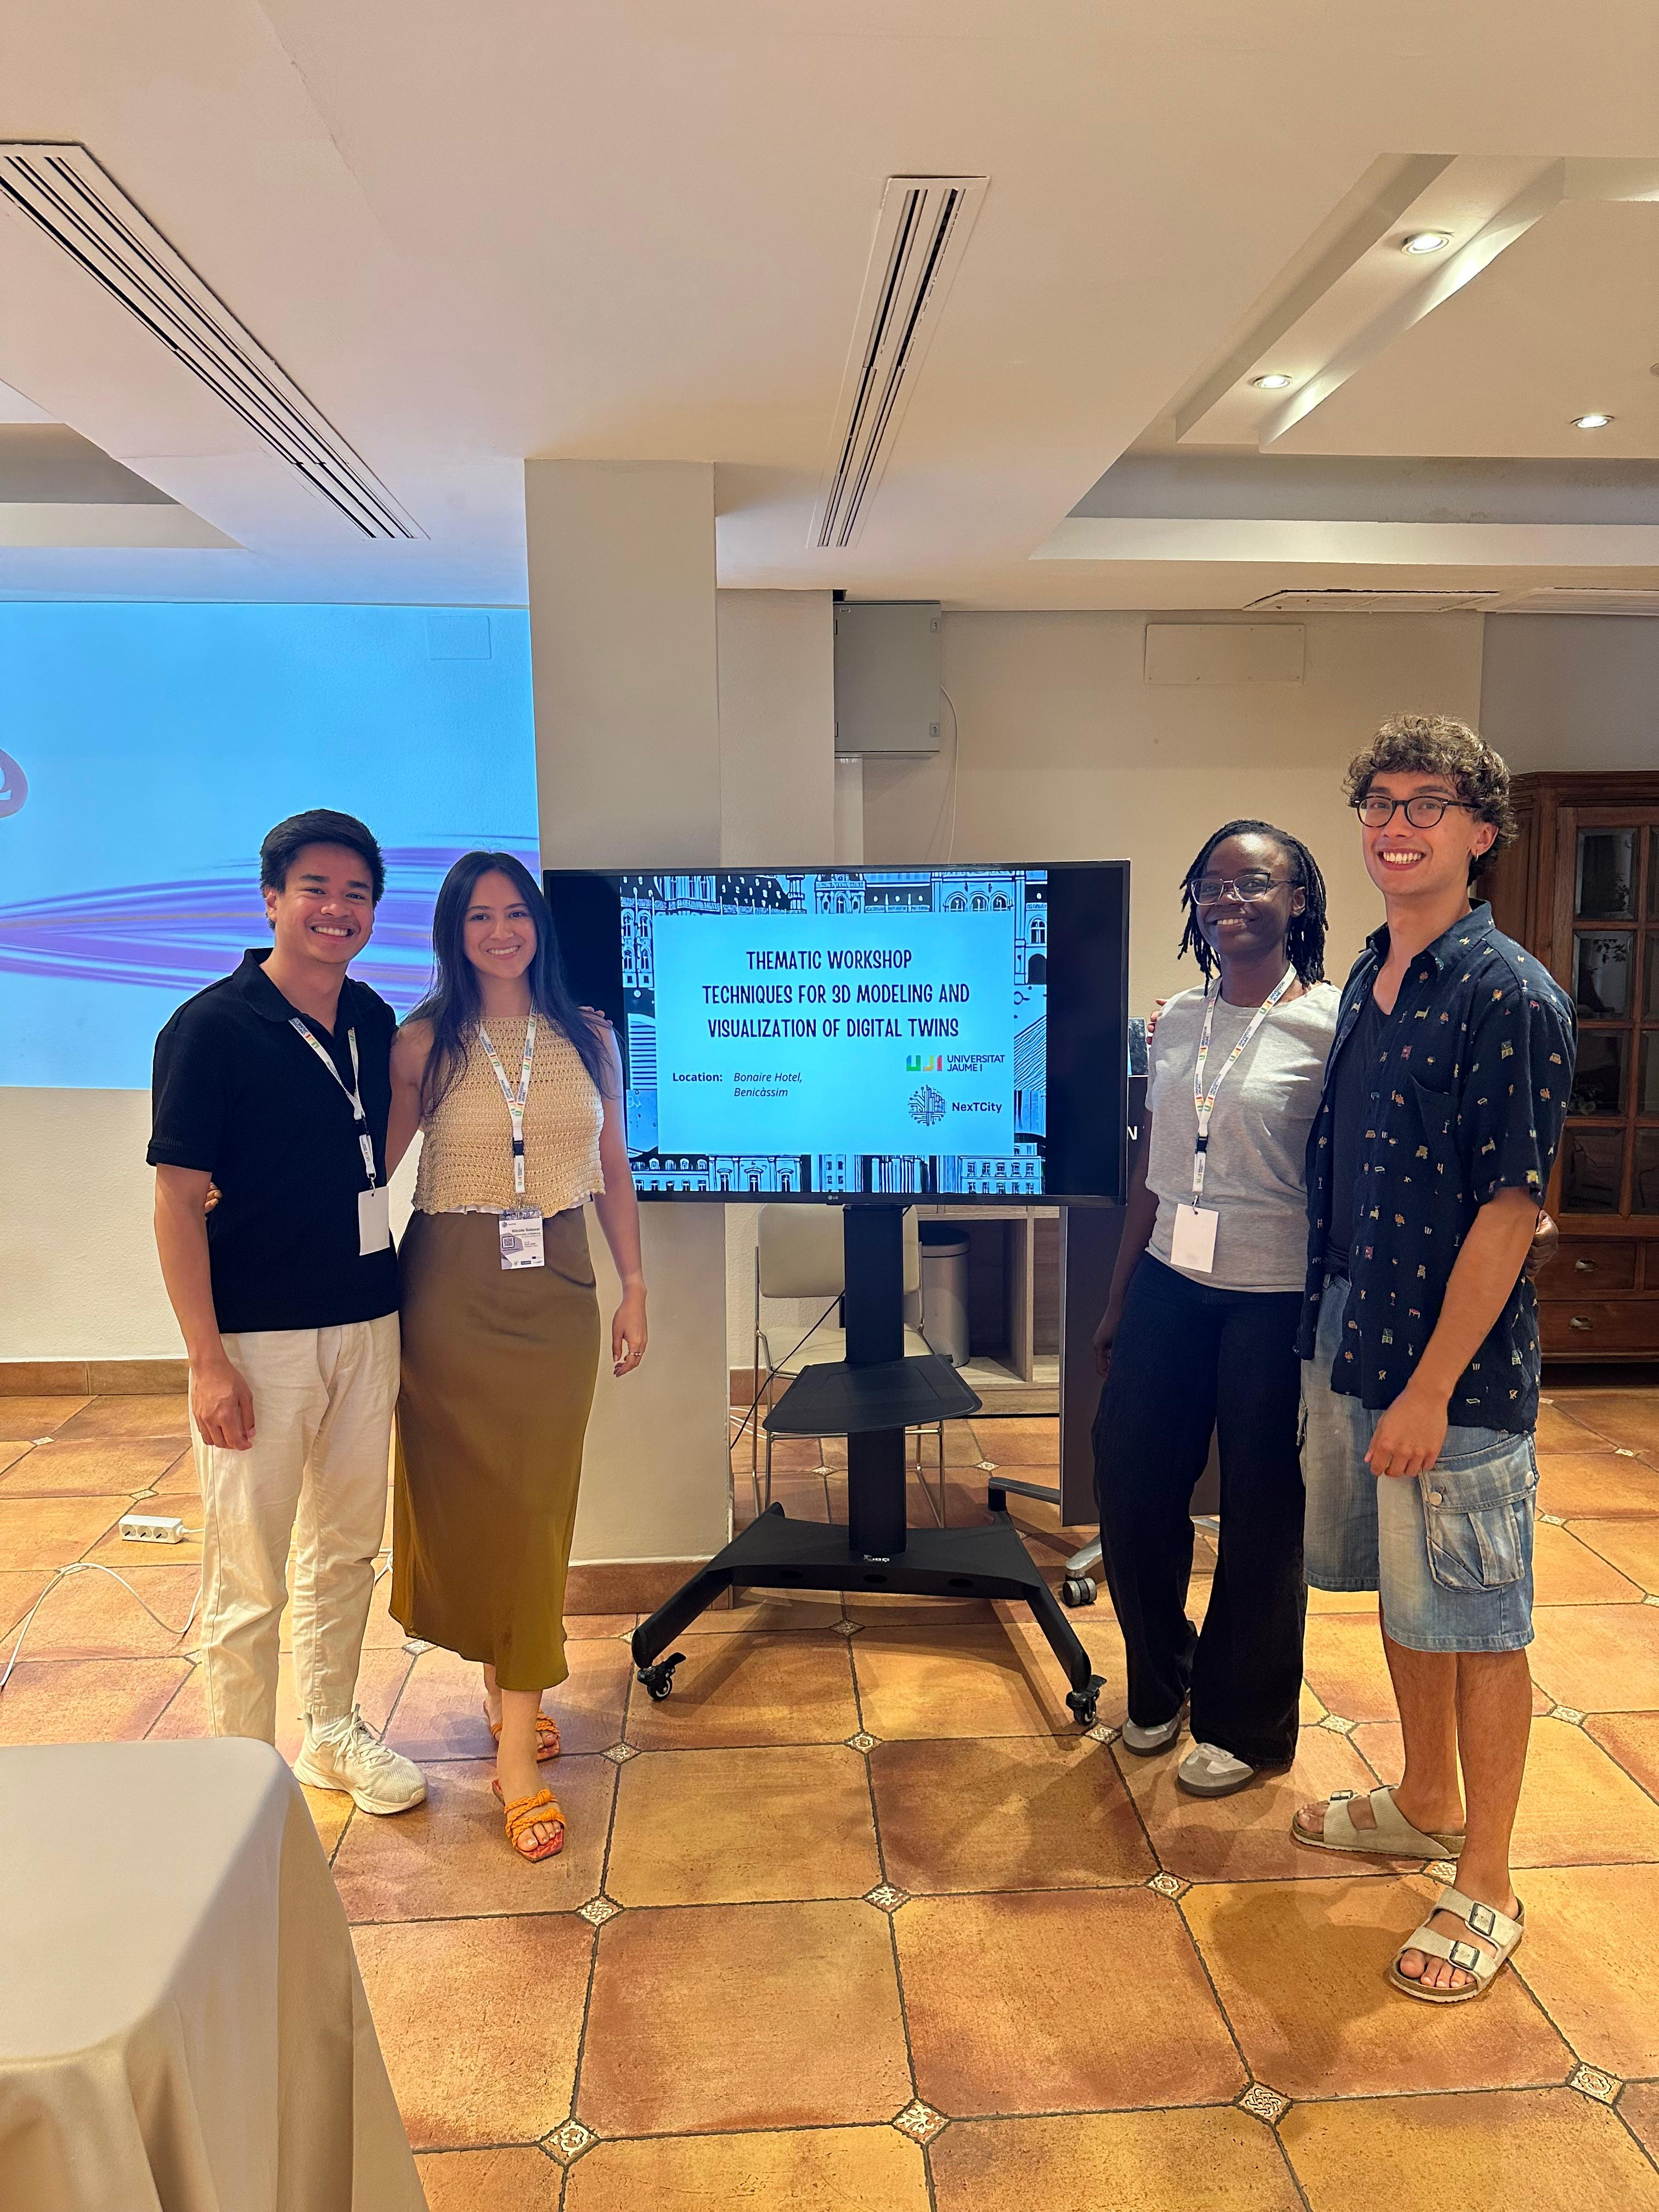
\includegraphics[width=3.30208in,height=\textheight]{images/erasmus peeps.jpg}

\hfill\break
\emph{Image 1: \href{https://www.linkedin.com/in/nicolesalazarc/}{Nicole
Salazar} and me (CDE students present)}

\emph{Image 2: With other EMJM+ students (the
\href{https://mastergeotech.info/}{Geotech} program)}
\end{quote}
\end{quote}




\end{document}
